\documentclass[12pt]{abnt}

\usepackage[utf8]{inputenc}
\usepackage[brazil]{babel}
\usepackage{graphicx}
\usepackage{color}
\usepackage[colorlinks,linkcolor=black,citecolor=black,urlcolor=black,plainpages=false,pagebackref,hyperfootnotes=false,pdfpagelabels]{hyperref}
\usepackage{framed}
\usepackage{listings} % para código fonte
\lstset{numbers=left,
language=C,
stepnumber=1,
firstnumber=1,
numberstyle=\tiny,
extendedchars=true,
breaklines=true,
frame=tb,
basicstyle=\footnotesize,
stringstyle=\ttfamily,
showstringspaces=false
backgroundcolor=\color{gray}
}
%\usepackage[portugues,boxed,lined]{algorithm2e}

%Para inserir o códigos fonte
\usepackage{float}   
\usepackage{fancyvrb}

%===== Códigos Fonte =====
\newenvironment{codeverbatim}{\VerbatimEnvironment \small
   \begin{Verbatim}[xleftmargin=20mm]}
   {\end{Verbatim}}
%=======
\floatstyle{boxed}  % tipos: plain, boxed, ruled
\newfloat{codigo}{tbp}{lop}[section]  % numera os captions com  número de seção.
\floatname{codigo}{Código}
% nome para ser usado no sumário
\newcommand{\listofcodename}{Lista de Códigos}
%=========================

\title{``Atividade pártica de Segurança de Dados''}

\author{Anderson de França Queiroz\\
Tiago de França Queiroz}

\date{Abril de 2012}

\begin{document}

\sloppy

\maketitle

\begin{titlepage}

  \vspace{6cm}

  \begin{flushleft}
    \sffamily\slshape
    ``If you don't stand for something,\\
	you'll fall for anything''\\
	(Filme Sucker Punch)
   
    \vspace{1cm}
    
    \end{flushleft}

\end{titlepage}

%\clearpage
\tableofcontents
\clearpage

\chapter{Descrição de um ataque}

Um atacante deseja tronar indisponível o acesso por SSH do servidor de um conhecido. O modo que ele escolhe para fazer é utilizar
um programa que ele desenvolveu para gerar requisições de conexção com o servidor initerruptamente partindo de vários computadores
diferentes, ou seja, um ataque de DDoS -- \textit{Distributed Denial-of-Service}.

A disponibilidade de serviço é muito importante para várias empresas, principalmente quando o produto que a empresa ofereçe é o serviço.
Ter um serviço indisponível pode causar perdas como: compras não serem realizadas (sites de e-commerce); clientes trocarem de empresa para uma cujos
serviços não fiquem indisponíveis; perda de confiabilidade; entre outras coisas.

Um ataque simples
que visa indisponibilizar serviço é o ataque de negação de serviço, DoS (\textit{Denial-of-Service}), 
esse tipo de ataque realiza um número muito grande
de requisições ao serviço em curto espaço de tempo, assim o servidor não consegue reponder a todos, o que gera indisponibilidade do sistema.
Existe a variante distribuida do DoS, o DDoS (\textit{Distributed Denial-of-Service}), 
que utiliza simultaneamente vários computadores para realizar ataques de DoS a um mesmo alvo.


No cenário descrito o atacante desenvolve um programa que chama o cliente padrão de SSH do sistema operacional e tenta logar no host alvo. O programa
apenas solicita a conexão, uma vez que o objetivo é apenas indisponibilizar o sistema e não invadi-lo.
De posse do programa ele vai a um laboratório de informica de sua universidade e instala o programa em todos os computadores de modo que
quando se faça o login o programa inicialize em background. Como é preciso apenas a senha de usuário para realizar essa operação e todos
os alunos utulizam o mesmo usuário, sempre que alguém logar no computador o ataque de DoS iniciará.

\chapter{Roteiro de ataque de DDoS}

O ataque de DDoS (\textit{Distributed Denial-of-Service}) que será estudado nesta aula objetiva indisponibilizar o serviço de SSH comumente
utulizado para acesso remoto a computadores. 

\section{Criando um programa de DoS}
\label{programa}

A negação de serviço consiste em muitas requisições em um curto intervalo de tempo, de modo que o servidor não consiga atender a todas. Então nesse
experimento criaremos um programa em linguagem C que utiliza \textit{multithread} para realizar inúmereas requisições \texttt{SSH} a um servidor.

\begin{enumerate}

	\item Abra o editor preferência, sugere-se a utulização do \texttt{VIM}. Em um terminal execute \texttt{vim};
	\item Digite o código \ref{DoS};
	\item Edite as macros \texttt{NUM\_TRHEADS, COMANDO, TEMPO e ESPERA}. Onde:
		\begin{itemize}
		
			\item \texttt{NUM\_TRHEADS:} é o número de threads que serão criadas, ou seja,
			o número de conexões simultâneas que serão realizadas pelo programa;

			\item \texttt{COMANDO:} é o comando que será executado, neste experimento usaremos o ssh,
			então coloque um nome de usuário (de perferência um que exista na máquina alvo) e o IP ou
			domínio da máquina;

			\item \texttt{TEMPO:} é a hora em que o ataque irá começar;

			\item \texttt{ESPERA:} é o tempo que o programa irá esperar antes de ser fechado e encerrar
			as threads que estão realizando o  DoS.

		\end{itemize}

	\item Salve com o nome \texttt{DoS.c} e saia do editor;
	\item Compile, para isso execute no terminal \texttt{cc DoS.c -o DoS -lpthread};

\end{enumerate}

%\begin{framed}
%	\lstinputlisting[title={Código}, language=C, label=DoS, caption={Programa para o DoS}, extendedchars=true]{../DDOS.c}
%\end{framed}

\renewcommand{\baselinestretch}{0.5}  % distância entre linhas
\begin{codigo}[!hbt]
   \tiny  % tamanho da fonte
      %\vspace{2mm}
      \VerbatimInput[xleftmargin=8mm,numbers=left,obeytabs=true]{DDOS.c}
   \caption{Código fonte em C para o DoS.}
   \label{DoS}
\end{codigo}

\clearpage

\section{Realizando o ataque}

O programa descirto na sessão \ref{programa} tem como objetivo mostrar o funcionamento de um ataque de
DoS ou DDoS (\textit{Distributed Denial of Service}). O DDoS é um ataque de DoS distribuido, ou seja,
executado por várias máquinas (preferêncialmente com conexões distintas a internet) simultâneamente.

Para realizar o ataque primeiro é preciso descobrir quais máquinas estão com a porta 22 (porta do ssh)
aberta, para isso utilize o nmap da seguinte forma: \textit{nmap -T4 192.168.1.0/24}, onde o 192.168.1.0
é o IP da rede alvo. Analize a saída
do nmap a procura de uma máquina com a porta 22 aberta e edite o programa como descirto na sessão \ref{programa}.

\renewcommand{\baselinestretch}{0.5}  % distância entre linhas
\begin{codigo}[!hbt]
   \tiny  % tamanho da fonte
      %\vspace{2mm}
      \VerbatimInput[xleftmargin=8mm,numbers=left,obeytabs=true]{nmap.txt}
   \caption{Exemplo de saída do \texttt{nmap}.}
   \label{nmap}
\end{codigo}

Observe que na linha 16 lindica que o \texttt{ssh} está rodando e a porta está aberta, então, localize os IPs que estão com a porta 22 
aberta e substitua o valor da macro \texttt{COMANDO} para \texttt{ssh USUÁRIO@IP\_COM\_PORTA\_22\_ABERTA}, em nosso exemplo seria
\texttt{ssh ufabc@192.168.1.5}. 

Rode no terminal o comando \texttt{ssh USUÁRIO@IP\_COM\_PORTA\_22\_ABERTA} e quando for perguntado se deve adicionar a chave reponda sim(yes).
Agora compile e execute o programa. Observe a saída do programa, o que ela indica?

É possível utilizar o \texttt{wireshark} para observar o tráfego da rede e ver o ataque acontecendo, para isso abra o \texttt{wireshark}
(em um terminal digite \texttt{sudo wireshark}). Na tela inicial localize a lista de interfaces de rede e escolha a interface conectada na
rede onde está sendo realizado o ataque, em nosso exemplo é a \texttt{wlan0}, como é mostrado na figura \ref{wireshark}.

Após selecionar a interface de rede a captura de pacotes inciará, então no campo \texttt{Filter} coloque \texttt{ip.dst == IP\_SOB\_ATAQUE},
em nosso exemplo seria \texttt{ip.dst == 192.168.1.5}, como pode ser visto na figura \ref{captura}. Assim apenas os pacotes endereçados
a máquina sob ataque irão aparecer. É possível identificar as requisições de conexão ssh? Existe apenas uma requisição ou várias?

\begin{figure}[!hbt]
  \centering
  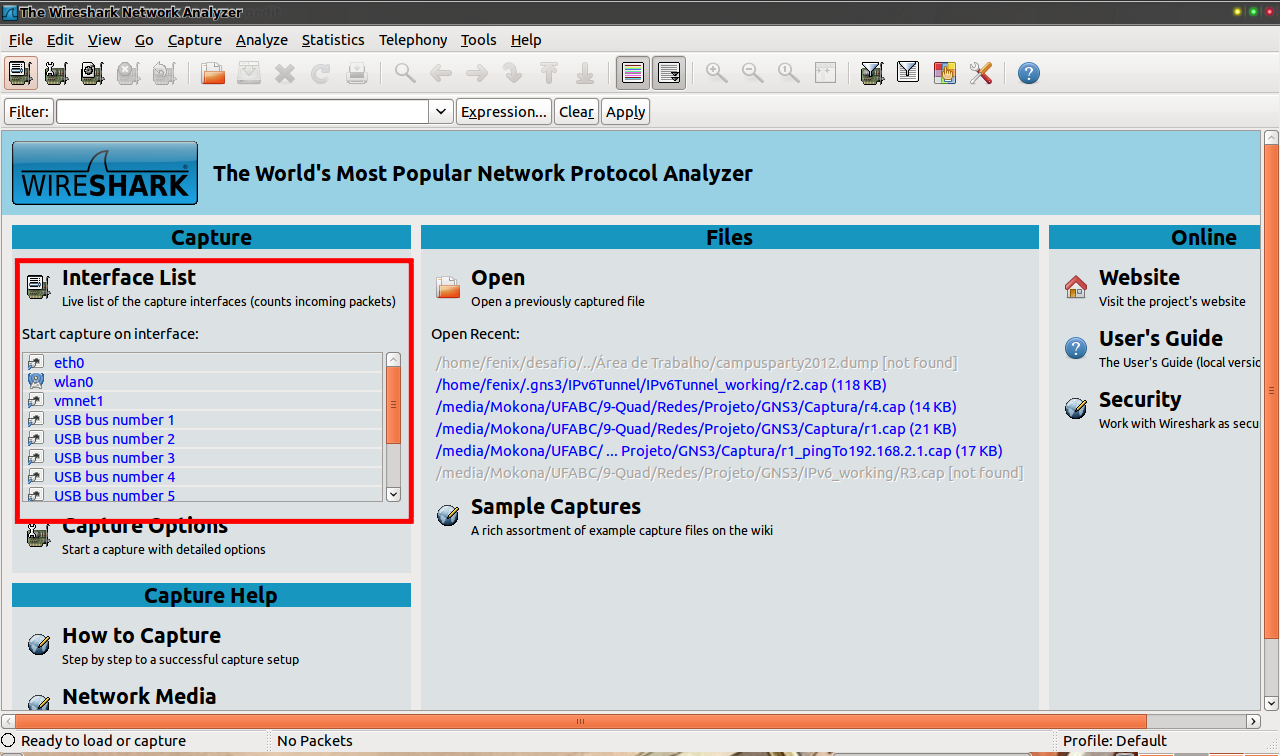
\includegraphics[scale=0.3]{Wireshark-s}
  \caption[Wireshark-s]{Selecionando interface conectada a rede no \textit{wireshark}.}
  \label{wireshark}
\end{figure}

\begin{figure}[!hbt]
  \centering
  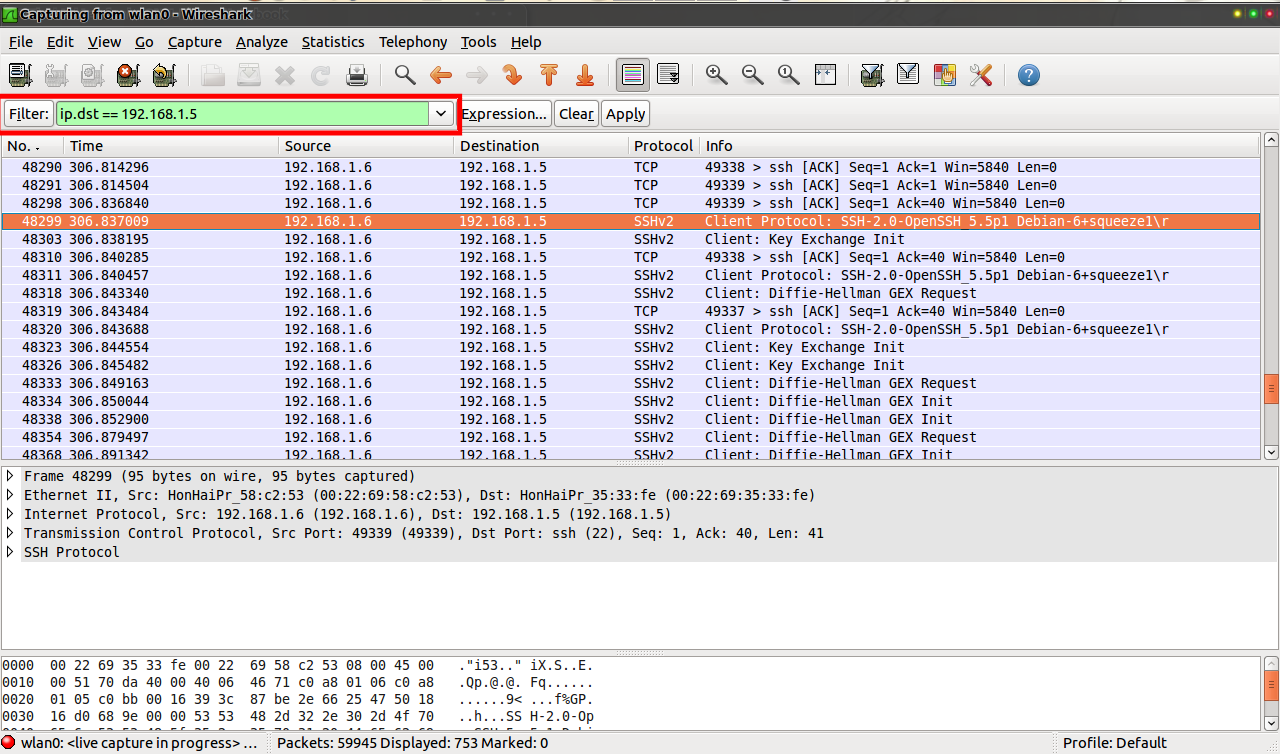
\includegraphics[scale=0.3]{Wireshark-cap}
  \caption[Wireshark-cap]{Filtrando pacotes no \texttt{wireshark}.}
  \label{captura}
\end{figure}




\chapter{Teste do Roteiro}
Primeiramente o namp foi executado para descobrir quais máquinas possuiam um servidor
ssh ativo, o resultado pode ser visto no código \ref{nmap}
A saída será similar a esta:

\renewcommand{\baselinestretch}{0.5}  % distância entre linhas
\begin{codigo}[!hbt]
   \tiny  % tamanho da fonte
      %\vspace{2mm}
      \VerbatimInput[xleftmargin=8mm,numbers=left,obeytabs=true]{saida.namp}
   \caption{Resultado o nmap.}
   \label{nmap}
\end{codigo}

Analizando o resultado do nmap percebe-se que a única máquina com o servidor
ssh ativo e a prota 22 aberta é a máquina de IP 192.168.1.6.

Editou-se o código \ref{programa} de modo que as macros ficaram da seguinte forma:
\begin{itemize}

	\item \texttt{ESPERA = 5};

	\item \texttt{NUM\_TRHEADS = 10};

	\item \texttt{COMANDO "ssh user@192.168.1.6"};

	\item \texttt{TEMPO "Mon 2012-05-07 23:25:00 BRT"};

\end{itemize}

O programa foi compilado e executado, obtendo-se a saída mostrada no código \ref{saidaDOS},
onde é possível perceber que foram executadas 10 tentativas de conexão por ssh.

\renewcommand{\baselinestretch}{0.5}  % distância entre linhas
\begin{codigo}[!htb]
   \tiny  % tamanho da fonte
      %\vspace{2mm}
      \VerbatimInput[xleftmargin=8mm,numbers=left,obeytabs=true]{saida.Dos}
   \caption{Resultado o nmap.}
   \label{saidaDOS}
\end{codigo}
\clearpage
\bibliography{relatorio}

\end{document}
